\documentclass[../../main.tex]{subfiles}

%-----------------------------------------------------------%
\begin{document}
\section{Feature Extraction}
\thispagestyle{fancy}

Feature Extraction is the process of obtaining the centroids of all detectable stars, with maximum accuracy. It takes in the image obtained by the image sensor and outputs the location of the corresponding centroid of various stars in image plane coordinate.

We are working on three different algorithms for Feature Extraction, and selection between them will be done on the basis of performance, time-wise and accuracy-wise (along with availability of resources in case of the sequential algorithms).
\begin{itemize}
    \item Sequential Algorithms:\\
    \ These will be implemented on the FPGA, provided that enough resources are left over after interfacing is implemented. We have two sequential algorithms that we plan to test on the FPGA:
    \begin{itemize}
        \item The pixel-by-pixel tagging algorithm:\\
        \ This algorithm goes through all the pixels in the image and assigns a tag to each pixel. Tags that get connected at a pixel are merged at the end of tagging. This is a modification of one of the classical algorithms used for image labelling. An example of how this labelling algorithm works is presented at \href{https://aishack.in/tutorials/labelling-connected-components-example/}{this webpage}.
        \item The run length encoding (RLE) algorithm:\\
        \ This algorithm compares the starting and ending points of continuous ranges of pixels in every row and assigns tags to those ranges. Tags that get connected to the same range are merged at the end of comparisons for each row. The algorithm to be implemented is presented in \cite{fe_blob_detection}.
    \end{itemize}
    \item Recursive Algorithms:\\
    We are working on a recursive centroiding algorithm called the region growth algorithm. Recursive algorithms can not be implemented on the FPGA as HLS can not synthesize recursive functions. Therefore, this algorithm will run on the microcontroller.
\end{itemize}

All three of these work on the basis of thresholding. The pixels with intensity above a pre-set threshold are said to be bright, and the algorithms define stars as 4-connected regions of bright pixels. 

Two pixels are said to be 4-connected if they share an edge. Thus, for a given pixel, the pixels to the immediate "north", left, right and "south" are said to be 4-connected to it and vice-versa. 4-connected regions can be defined quite easily using this definition.

There are lower and upper bounds on the number of pixels in each star to account for anomalous readings and large celestial bodies that are not stars and hence can't be matched by the star matching algorithms.

These constants and their tentative values are listed in the following table:

\begin{table}[h]
    \centering
    \begin{tabular}{|c|c|}
        \hline
        \textbf{Constant} & \textbf{Tentative Value}\\
        \hline
        Threshold & 20\\
        star\_min\_pixel & 3 \\
        star\_max\_pixel & 120\\
        \hline
    \end{tabular}
    \caption{Constants used for feature extraction}
    \label{tab:fe_const}
\end{table}

\large{\textbf{Finding the centroid for each star:}}\\
\normalsize
There are two centroiding methods which are commonly employed by star trackers:
Center of gravity and Gaussian curve fitting.

\textbf{Gaussian Curve Fitting:}
The pattern of light caused by a single star on the image plane can be approximated as a 2D Gaussian function. Gaussian curve fitting attempts to fit a Gaussian function to the pattern of light caused by each star. Once this is achieved, the centroid of the star can be found by calculating the location of the fitted Gaussian function's peak. This is the more accurate of the two methods.

\textbf{Center of Gravity:}
Compared to Gaussian curve fitting, a Center of gravity equation is less accurate, but is much less processor-intensive and so we face a trade-off between the time taken by the process and its accuracy and which process is to be employed must be decided based upon the system's requirements.

According to the center of gravity approach, the centroid of each each star is defined as
\begin{equation}
\boxed{
\begin{aligned}
    C_{x} & := \frac{\sum C_{i_{x}}Intensity_{i}}{\sum Intensity_{i}}\\
    C_{y} & := \frac{\sum C_{i_{y}}Intensity_{i}}{\sum Intensity_{i}}
\end{aligned}
}
\end{equation}
There are other alternate formulae similar to this one, presented in \cite{zhang2011star}, as follows:
\begin{equation}
\boxed{
\begin{aligned}
    C_{x} & := \frac{\sum C_{i_{x}}(Intensity_{i}-Threshold)}{\sum (Intensity_{i}-Threshold)}\\
    C_{y} & := \frac{\sum C_{i_{y}}(Intensity_{i}-Threshold)}{\sum (Intensity_{i}-Threshold)}
\end{aligned}
}
\end{equation}
\begin{equation}
\boxed{
\begin{aligned}
    C_{x} & := \frac{\sum C_{i_{x}}Intensity^2_{i}}{\sum Intensity^2_{i}}\\
    C_{y} & := \frac{\sum C_{i_{y}}Intensity^2_{i}}{\sum Intensity^2_{i}}
\end{aligned}
}
\end{equation}
\begin{equation}
\boxed{
\begin{aligned}
    C_{x} & := \frac{\sum C_{i_{x}}(Intensity_{i}-Threshold)^2}{\sum (Intensity_{i}-Threshold)^2}\\
    C_{y} & := \frac{\sum C_{i_{y}}(Intensity_{i}-Threshold)^2}{\sum (Intensity_{i}-Threshold)^2}
\end{aligned}
}
\end{equation}


In the Gaussian fitting algorithm, an initial centroid is found out using the Center of gravity method, then the pixels are assigned an additional weight which is given by Gaussian probability distribution function.

We have (for now) decided to go with the the center of gravity approach because of the simplicity and the computational cost of implementing the Gaussian Curve Fitting algorithm.

Currently, the pixel-by-pixel algorithm and the region growth algorithm have been coded and tested on both MATLAB and C++. These testing results have been compiled and presented in section \ref{sec:Electrical_test}.

We now present the details of the algorithms.

\subfile{Chapters/Electrical/pixel_by_pixel}
\subfile{Chapters/Electrical/runLengthEncoding}

\begin{Flowchart}
    \centering
    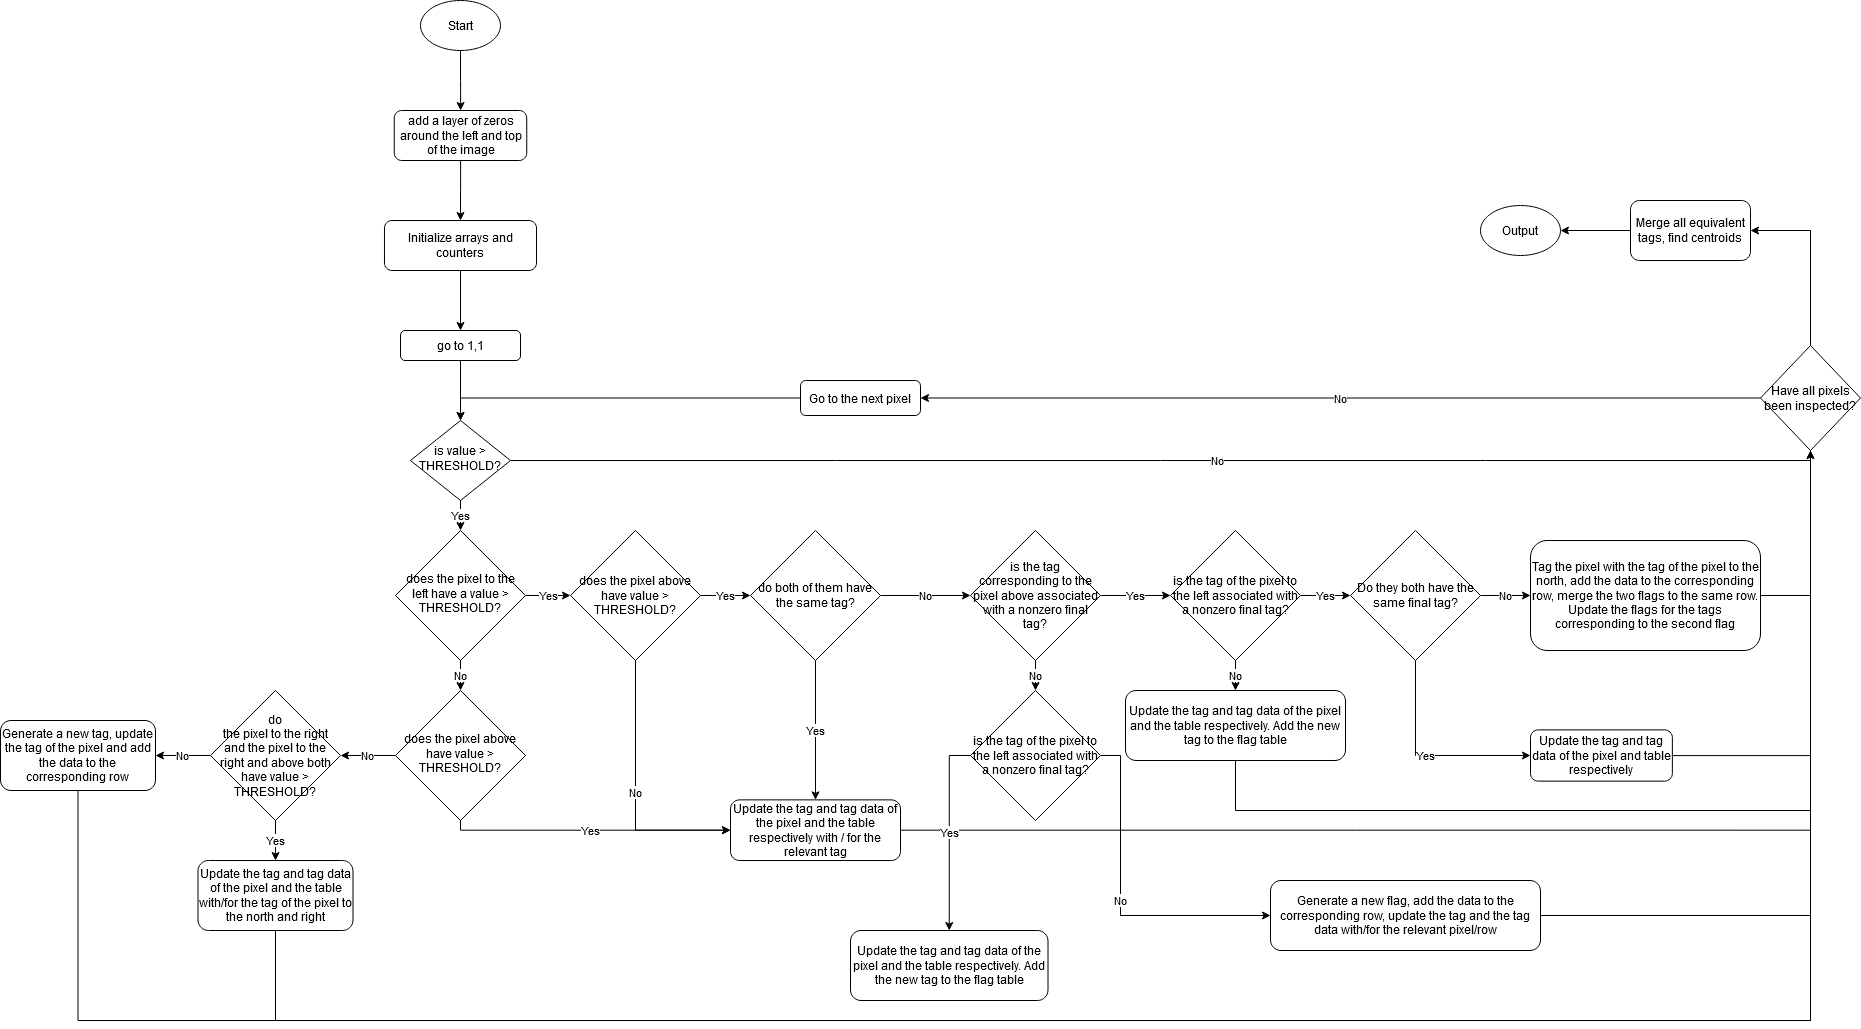
\includegraphics[width=\textwidth]{Figures/Electrical/centroiding_2_non_coding.png}
    \caption{Pixel-by-Pixel Tagging Algorithm}
    \label{FC:pbp_centroiding}
\end{Flowchart}

\begin{Flowchart}
    \centering
    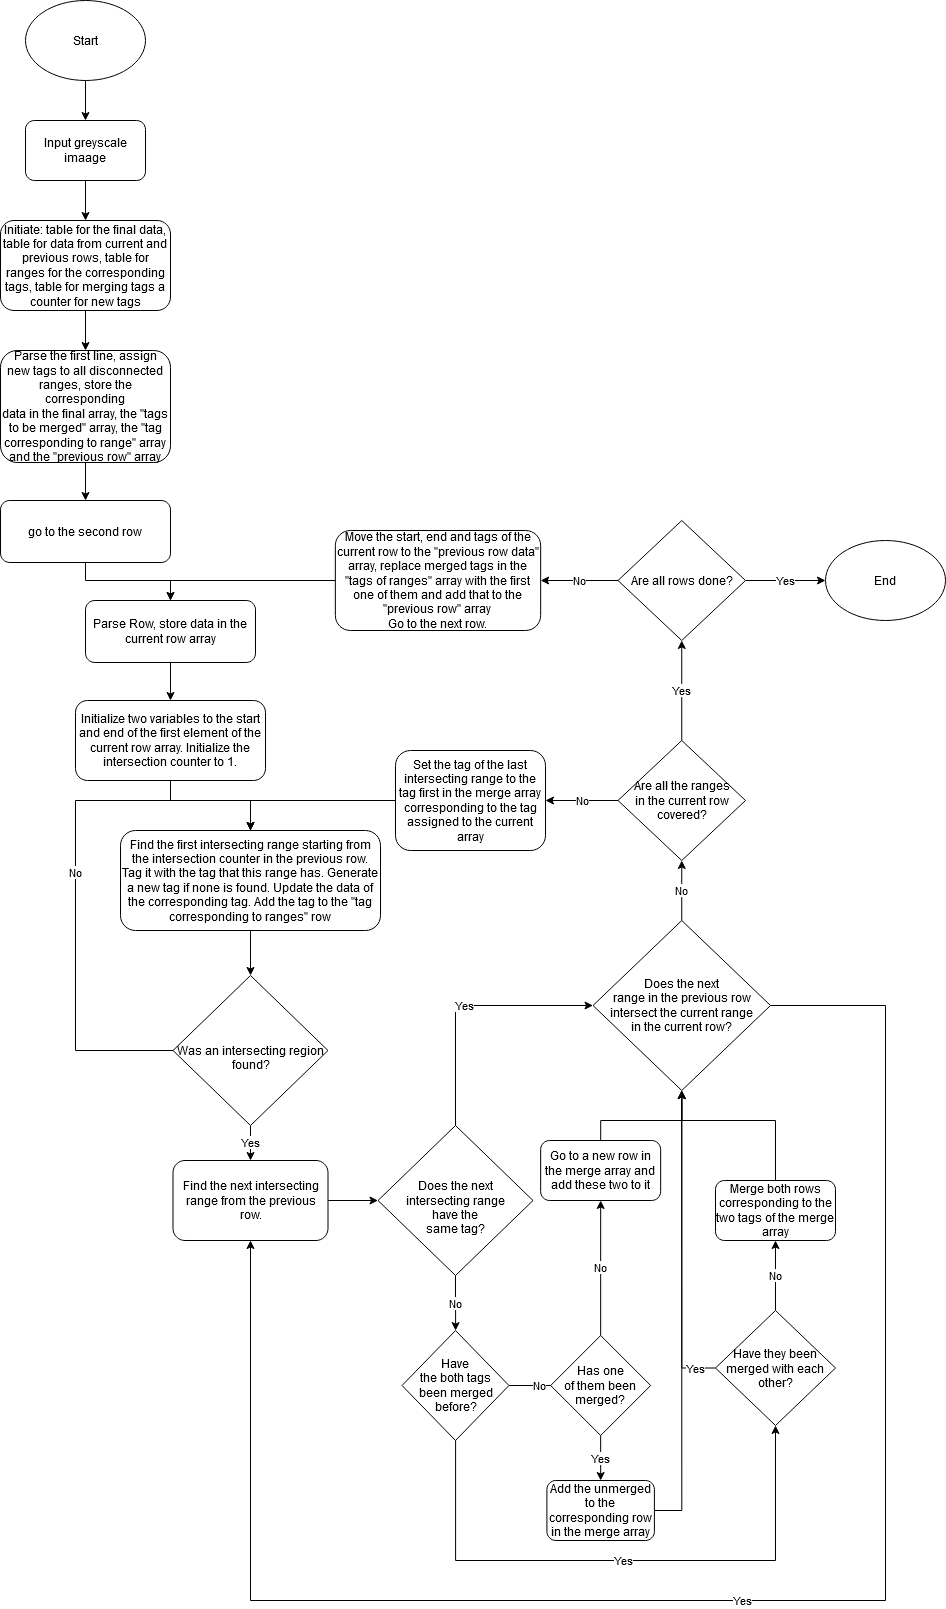
\includegraphics[width = 0.7\textwidth]{Figures/Electrical/centroiding_3.png}
    \caption{Run Length Encoding Algorithm}
    \label{FC:flow_fe_rle}
\end{Flowchart}
%----------------------------END----------------------------%
\end{document}